%%%%%%%%%%%%%%%%%%%%%%%%%%%%%%%%%%%%%%%%%
% Thin Sectioned Essay
% LaTeX Template
% Version 1.0 (3/8/13)
%
% This template has been downloaded from:
% http://www.LaTeXTemplates.com
%
% Original Author:
% Nicolas Diaz (nsdiaz@uc.cl) with extensive modifications by:
% Vel (vel@latextemplates.com)
%
% License:
% CC BY-NC-SA 3.0 (http://creativecommons.org/licenses/by-nc-sa/3.0/)
%
%%%%%%%%%%%%%%%%%%%%%%%%%%%%%%%%%%%%%%%%%

%----------------------------------------------------------------------------------------
%	PACKAGES AND OTHER DOCUMENT CONFIGURATIONS
%----------------------------------------------------------------------------------------

\documentclass[a4paper, 21pt]{article} % Font size (can be 10pt, 11pt or 12pt) and paper size (remove a4paper for US letter paper)

\usepackage[protrusion=true,expansion=true]{microtype} % Better typography
\usepackage{graphicx} % Required for including pictures
\usepackage{wrapfig} % Allows in-line images
\usepackage[utf8]{inputenc}  % UTF8 characters
\DeclareGraphicsExtensions{.pdf,.png,.jpg}
\graphicspath{{logos/}{figs/}}
\usepackage{caption}
\usepackage{mathpazo} % Use the Palatino font
\usepackage[T1]{fontenc} % Required for accented characters
\usepackage{url} % For URLs
\usepackage{listings}        % code listings
\usepackage{color} 
\usepackage{float}  
\linespread{1.05} % Change line spacing here, Palatino benefits from a slight increase by default

\makeatletter
% \renewcommand\@biblabel[1]{\textbf{#1.}} % Change the square brackets for each bibliography item from '[1]' to '1.'
\renewcommand{\@listI}{\itemsep=0pt} % Reduce the space between items in the itemize and enumerate environments and the bibliography

\renewcommand{\maketitle}{ % Customize the title - do not edit title and author name here, see the TITLE block below
\begin{flushright} % Right align
{\LARGE\@title} % Increase the font size of the title

\vspace{50pt} % Some vertical space between the title and author name

{\large\@author} % Author name
\\\@date % Date

\vspace{40pt} % Some vertical space between the author block and abstract
\end{flushright}
}

%----------------------------------------------------------------------------------------
%	TITLE
%----------------------------------------------------------------------------------------

\title{\textbf{Handbook for Matlab GUI}\\ % Title
Positioning Algorithms Comparison} % Subtitle

\author{\textsc{Pablo del Hoyo Rodríguez} % Author
\\{\textit{Technische Universität Hamburg-Harburg}}} % Institution

\date{\today} % Date

%----------------------------------------------------------------------------------------

\begin{document}

\maketitle % Print the title section

%----------------------------------------------------------------------------------------
%	ABSTRACT AND KEYWORDS
%----------------------------------------------------------------------------------------

%\renewcommand{\abstractname}{Summary} % Uncomment to change the name of the abstract to something else

\begin{abstract}
This document presents the detailed information about the program used to compare some of the localization algorithms. The program consists of a Graphical User Interface (GUI) for Matlab which easily set a real case scenario and presents the data gathered by Pozyx device mounted on an Arduino board. The GUI provides a pop-up menu where an algorithm can be chosen in order to compare the estimated position. Also, it may localize an agent in real time, tracking the position of the Arduino board.  
\end{abstract}

\hspace*{3,6mm}\textit{Keywords:} Matlab, GUI, Arduino, Pozyx, Positioning, Algorithm % Keywords

\vspace{30pt} % Some vertical space between the abstract and first section

\tableofcontents
\newpage
%----------------------------------------------------------------------------------------
%	ESSAY BODY
%----------------------------------------------------------------------------------------

\section{Prerequisites}

%This statement requires citation \cite{Smith:2012qr}; this one does too \cite{Smith:2013jd}. Lorem ipsum dolor sit amet, consectetur adipiscing elit. Aenean dictum lacus sem, ut varius ante dignissim ac. Sed a mi quis lectus feugiat aliquam. Nunc sed vulputate velit. Sed commodo metus vel felis semper, quis rutrum odio vulputate. Donec a elit porttitor, facilisis nisl sit amet, dignissim arcu. Vivamus accumsan pellentesque nulla at euismod. Duis porta rutrum sem, eu facilisis mi varius sed. Suspendisse potenti. Mauris rhoncus neque nisi, ut laoreet augue pretium luctus. Vestibulum sit amet luctus sem, luctus ultrices leo. Aenean vitae sem leo.
As the program will provide a communication between the Arduino board and the computer, two parts will be considered in order to make the installation the Matlab side and the Arduino side:\\
\begin{figure}[!hbbp]
\begin{center}

\includegraphics[scale=0.8]{fig/matlab_arduino.png}
\end{center}
\caption{Both sides of the program}
\end{figure}

For the Matlab site it is required:
\begin{itemize}
\item Matlab R2016a (older versions may be valid)
\item Arduino Support from Matlab: package to communicate with an Arduino. The installation steps are available at reference \cite{Matlab:Arduino} and is usually installed by double clicking the package download file.
\end{itemize}

For the Arduino side is required:
\begin{itemize}
\item Arduino Uno x1
\item USB-B Cable x1
\item Pozyx Shield for Arduino
\item  The Arduino IDE and Pozyx Arduino Library: the installation steps are provided at reference \cite{Arduino:Started}
\item Pozyx Anchor x[3, 6]
\item  USB-C Cable x[3, 6]
\end{itemize}

%------------------------------------------------

\section{Script Files}
The localize.zip file is provided with the following files:
\begin{table}[!httpb]
\centering
\begin{tabular}{|l|l|}
\hline
\textbf{File}            & \textbf{Description}                                                                                                                                         \\ \hline
HandbookLocalize.pdf     & This file, description and a tutorial of the program                                                                                                         \\ \hline
\textbf{localize.m}               & Main Matlab file. To be executed                                                                                                                             \\ \hline
localize.fig             & Matlab Figure for the GUI                                                                                                                                    \\ \hline
positioning\_arduino.ino & \begin{tabular}[c]{@{}l@{}}Scketch to run onto the Arduino, do the localization\\ See section \ref{se:arduino} for more details\end{tabular}               \\ \hline
(subfolder) functions    & Some Matlab functions including these below                                                                                                                  \\ \hline
changeVisibility.m       & Hide buttons during execution to prevent errors                                                                                                    \\ \hline
displayAnchors.m         & Plot the anchors                                                                                                                                             \\ \hline
initArduino.m            & Initialize a serial communication Matlab-Arduino                                                                                                     \\ \hline
presentBP.m              & \begin{tabular}[c]{@{}l@{}}Plot the estimated position for Non-Parametric\\ Belief Porpagation (BP) algorithm. See \cite{BP} \end{tabular} \\ \hline
presentInfo.m            & \begin{tabular}[c]{@{}l@{}}Split the information read by the Arduino.\\ Calulates the Pozyx position.\end{tabular}                                           \\ \hline
presentPozyx.m           & \begin{tabular}[c]{@{}l@{}}Plot the estimate position for Pozyx algorithm.\\ See \cite{Pozyx:localize} for more details\end{tabular}                      \\ \hline
setAnchors.m             & Present the information read by the anchors                                                                                                                  \\ \hline
updatePorts              & Update the communication ports available (USB)                                                                                                               \\ \hline
(subfolder) functionsBP  & Several functions to calculate the BP solution                                                                                                               \\ \hline
\end{tabular}
\caption{List of files}
\label{tab:list_of_files}
\end{table}
\newpage
%------------------------------------------------


\section{Arduino Setup}\label{se:arduino}
Before running the main Matlab file (\textit{localize.m}), some restrictions about the scenario have to be taken into consideration:
\begin{itemize}
\item First and most important, the identifiers of the anchors must be specified in the sketch \textit{positioning\_arduino.ino}. The number of anchors must be comprised between three and six anchors. The external library does not support fewer or more anchors, so it is out of the scope of the program to work with another amount of anchors. This can be done by editing the following lines:
\begin{lstlisting}[language=c, breaklines=true, commentstyle=\color{blue}, basicstyle=\ttfamily\small]
// Edit with your devices:
uint8_t num_anchors = 4;
uint16_t anchors[4] = {0x6F13, 0x6F17, 0x6F23, 0x6F24};
\end{lstlisting}
\item Only one tag is possible. This is due to the calibration algorithm, which considers every tag as an anchor. The distance to the tag could be gotten as well as its coordinates. This means that the tag would behave indistinctly to an anchor. Consequently, only non-cooperative algorithms are possible.
\item The first anchor would define the origin of the coordinates map as the position (0,0). The second one would define the x axis and the third one the y axis, so it is desirable to put them as orthogonal as possible. This has to be taken into consideration if only positive coordinates and a more intuitive map are desired. It is also strongly recommended to separate all the devices at least a minimum distance (around 0.2 meters). If not, some errors in calibration may appear. Nevertheless, it is contemplated negative coordinates and not orthogonal axis. Again, section \cite{Pozyx:localize} is referred in order to get more information.
\item Coverage between all the devices involving the scenario is assumed. The Pozyx devices have a range coverage of about 100 meters in LOS conditions, so larger distances or other conditions have been not contemplated.
\item The process of the calibration is automatically done. In any case, the doc explains that the coordinates of the anchors can be manually set too if the coordinates are specified (in mm) and some code is uncommented as the following lines show:
\begin{lstlisting}[language=c, breaklines=true, commentstyle=\color{blue}, basicstyle=\ttfamily\small]
// only required for manual anchor calibration. 

  int32_t anchors_x[4] = {0, 1000, 0, 2000}; 
  int32_t anchors_y[4] = {0, 0, 1000, 2000};

// ...

// comment out the doAnchorCalibration if you are using manual mode

  SetAnchorsManual();
  
\end{lstlisting}
\end{itemize}

%------------------------------------------------
\section{Overview}
Once all the previous sections have been explained, the procedure to run the interface is described. The file localize.m has to be opened (by double-clicking or with the Matlab interface). After setting the path to the one corresponding to this project, the file can be executed (F5). This will open the interface, whose appearance is shown in the screenshot below:\\

\begin{figure}[H]
\begin{center}
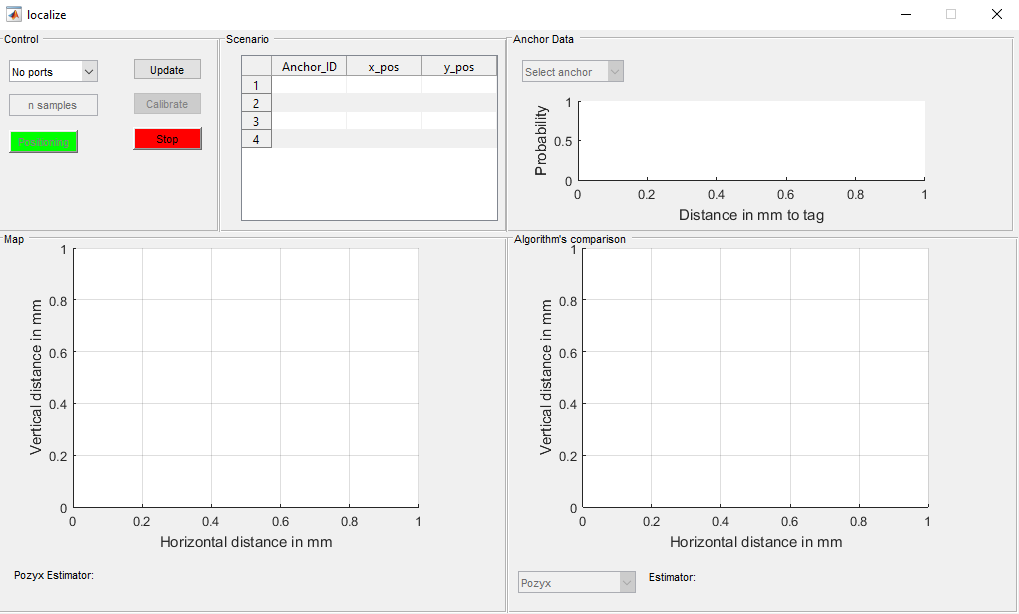
\includegraphics[scale=0.45]{fig/ss_ov.png}
\end{center}
\caption{The interface of the program running on Windows 10.}
\end{figure}

Five areas can be distinguished. The next sections indicates the functionalities for each one.
%------------------------------------------------


\section{Control}
This panel is in charge of the problem setup. Mainly is here where the options of the program are. The buttons are shown and explained above:
\begin{figure}[!hbbp]
\begin{center}
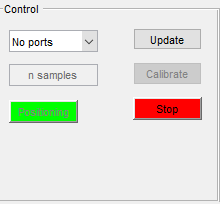
\includegraphics[scale=1.3]{fig/ss_control.png}
\end{center}
\caption{The control panel.}
\end{figure}

\begin{itemize}
\item The list of ports pop-up: indicates the currently connected COM ports. In case that nothing is connected, the execution of the code is not permitted. \textbf{Please make sure that the selected COM port is the one corresponding to the Arduino running the \textit{positioning\_arduino.ino} sketch}.
\item The update button: as its name indicates, updates the available ports and enable the buttons if at least one is connected:
\begin{figure}[H]
\begin{center}
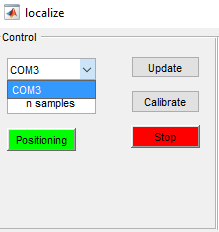
\includegraphics[scale=.9]{fig/ss_control2.png}
\end{center}
\caption{Setting the port after updating the list.}
\end{figure}
\item n samples text box: this sets the number of samples that will be used for the localization algorithms. For the case of the Pozyx algorithm, this number will set the times that the device is localized (to calculate its mean). For the case of BP, this number will set the number of messages that the tag will exchange with each anchor. The default value is 20, so if nothing is changed the tag will determine 20 estimators to each anchor, being part of the input data for the algorithm (more info in \ref{se:ad}. \textbf{Please make sure that only positive integers are considered}. Other values may arise unconsidered errors. Also notice that larger values produces longer calculation times.
\item the calibrate button: it sends to the tag a command to automatically (by default) calibrate the position of the anchors. When the calibration is done the coordinates are plotted whit each anchor’s identification. Also, it gets the position of the tag during the specified samples according to the Pozyx algorithm, showing the current progress. After gathering these positions as (x,y) coordinates in millimetres, it plots its mean and also the scenario table is updated (see \ref{se:sc}). Once this process is successfully completed, both sections Anchor Data(\ref{se:ad}) and Algorithm's Comparison(\ref{se:ac}) will be available. \textbf{Please make sure that the devices are as fixed as possible during the calculation}.
\item the positioning button: it has a very similar behaviour to the previous button, as the calibration of the anchors is done and plotted. However, it shows a real time positioning of the device during the number of samples specified. Nevertheless, it does not provide data for the Algortihm's Comparison.
\item the stop button: interrupts the execution of the code, for example in the case a very large number of samples was set and the process is wanted to be closed. Pressing this button will consider the calibration as unsuccessful and no comparison will be available. It is recommended pressing the update button afterwards to restart it as the interruption may produce some synchronization issues in the serial communication.
\end{itemize}

%------------------------------------------------

\section{Scenario}\label{se:sc}
This section summarizes the scenario \textbf{after a calibration} is performed. The table contains the id, x position and y position (in mm) for every anchor detected in the area. If the manual calibration was selected, these data will be the same that the introduced in the sketch:
\begin{figure}[H]
\begin{center}
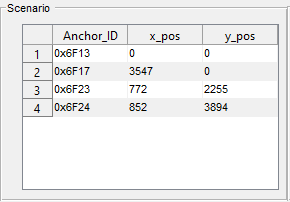
\includegraphics[scale=1.2]{fig/ss_sc.png}
\end{center}
\caption{Table scenario after a 4 anchors calibration.}
\end{figure}
%------------------------------------------------

\section{Map}
This section is available for both the calibration and positioning functions. For the first case, it will basically plots the information of the scenario table, with the anchors as red dots (showing their ids), plus the position estimated by the Pozyx device as a blue x. A text below displays the estimated position.\\

For the positioning function, a number of x equal to the number of samples will be plotted in real time, but in this case the data is not valid for the algorithms (as is assumed no to be fixed).

\begin{figure}[H]
\begin{center}
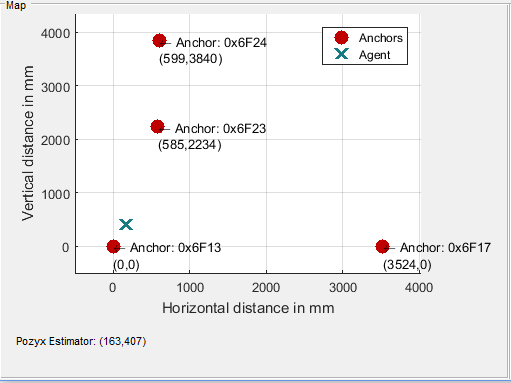
\includegraphics[scale=.8]{fig/ss_map.png}
\end{center}
\caption{Map scenario after a 4 anchors calibration with the Pozyx estimated position.}
\end{figure}
%------------------------------------------------

\section{Anchor Data}\label{se:ad}
This section is available once the calibration is performed. Each anchor can be selected with a pop-up menu, showing a list of (number of samples) estimators  to the agent. It is plotted the distribution of these distances (histogram), as well as its mean and variance. This will serve as the messages exchanged between the tag and the anchors.

\begin{figure}[H]
\begin{center}
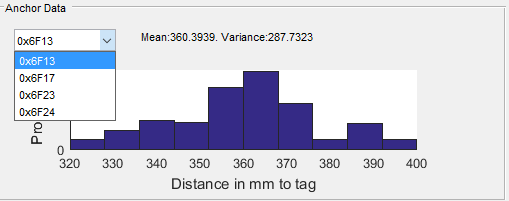
\includegraphics[scale=.9]{fig/ss_ad.png}
\end{center}
\caption{Anchor data: distribution of the distances between the tag and 0x6F13. Seems to be Gaussian.}
\end{figure}
%------------------------------------------------

\section{Algorithms Comparison}\label{se:ac}
This section is available once the calibration is performed. Each algorithm can be selected with a pop-up menu. For the Pozyx case (the default one), no calculation is required and it is the same the agent position in the map. For the BP, a calculation is required (which can take some time depending on the number of samples) and after finishing, the solution point is plotted and displayed.\\
\begin{figure}[H]
\begin{center}
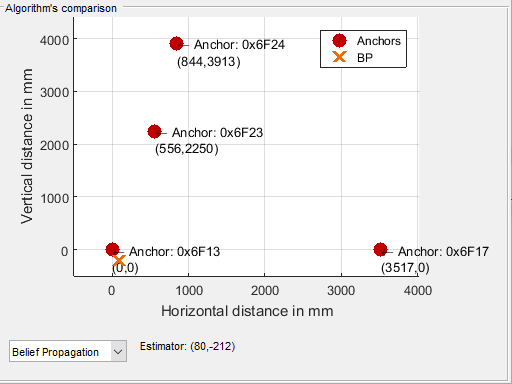
\includegraphics[scale=.8]{fig/ss_ac.png}
\end{center}
\caption{Map scenario with the BP solution coordinates. It can be compared with the Pozyx one.}
\end{figure}

Note that the progress of this algorithm can be followed on the console. It will provide different results after each execution and some other parameters regarding these calculations may be set in the code, especially in the file \textit{presentBP.m}:
\begin{lstlisting}[language=matlab, breaklines=true, commentstyle=\color{blue}, basicstyle=\ttfamily\small]
% Sim Data 
[simData.NSAMPLES, ~] = size(simTopology.msg);

simData.SIGMA = 0.1;
simData.ERROR_TYPE = 'Gaussian'; % 'Gaussian', 'Exponential', 'Uniform'
simData.NUM_ITERATIONS = 3;
simData.SAMPLE_TECHNIQUE = 'Importance'; % 'Importance', 'Mixture', 'Gibbs'
simData.K_MIXTURE_PARAMETER = 300; % Only in mixture: Max value is the number of devices + 1 is connected a device
simData.RESAMPLE_OPTION = 0; % Only in Importance: 0-yes, 1-no
simData.MULTIPLICATION_OPTION = 0; % 0-2on2 1-all together
simData.BMS_OPTION = 0; %Bandwidth Matrix Selector from 0 to 16
simData.SIMULATION_ITERATIONS = 1;
  
\end{lstlisting}
%------------------------------------------------

\section{Future Work}
Once the program has been presented, it has been observed that many functionalities can be implemented with the interface.\\

First thing would be to add more algorithms. As two of them have already been implemented, it seems easy to provide more of them if the code is already programmed. The only matter is to adapt it in order to present it onto the handles structure.\\

Also, it would be interesting to provide a tool to manually set the coordinates of the anchors, either using the table or by clicking the map.\\

The option of multiple agents can be considered too, but omitting the fact the agent provides its coordinates. Nevertheless, the library only supports a maximum of 6 anchors so not really complex scenarios would be considered though. Dealing with devices that are not in coverage between them presents a difficult challenge, as the devices should be at a physical distance of more than 100 m.\\

Also, some synchronization issues have been observed, as the data is read faster in some computers. If there is no data to be read, the code waits a time until it is again available, defining a buffer. However, it has been observed some unsuitability with these waiting times. Improve this buffer to work correctly in every scenario and computer is an important issue to be solved.\\

Finally, it is suggested to do experiments using this interface, studying the behaviour of the algorithms under different circumstances.

%----------------------------------------------------------------------------------------
%	BIBLIOGRAPHY
%----------------------------------------------------------------------------------------

\bibliographystyle{unsrt}

\bibliography{sample}

%----------------------------------------------------------------------------------------

\end{document}